% degree=[master]                             % 必选,学位类型
% language=[chinese|english],                 % 可选(默认:chinese),论文的主要语言
% review=[true|false]					      % 可选,盲审,默认为false
% bibstyle=[gb7714-2015|gb7714-2015ay|ieee],  % 可选(默认:gb7714-2015),参考文献样式
\documentclass[degree=master, language=chinese, review=false, oneside, AutoFakeBold]{shmtuthesis}

% 所有其它可能用到的包都统一放到shmtuthesis.sty中,可以根据自己的实际添加或者删除。
\usepackage{shmtuthesis}

% 定义图片文件目录与扩展名
\graphicspath{{figures/}}
\DeclareGraphicsExtensions{.pdf, .eps, .png, .jpg, .jpeg}

% 导入参考文献数据库
\addbibresource{thesis.bib}

% 论文信息,必须
\title{船岸连接}
\entitle{Ship Shore Connection}
\degreecategory{专业学位}
\author{辛浩东}
\enauthor{John Xin}
\studentid{202030210206}
\supervisor{耿攀}
\ensupervisor{Pan Geng}
\major{能源动力}
\enmajor{Electrical Engineering and Automation}
\finisheddate{二〇二一年二月}

\begin{document}
	
	% 无编号内容:论文封面、授权页
	\maketitle
	\makeDeclareOriginality
	\makeDeclareAuthorization
	
	% 使用罗马数字对前言编号
	\frontmatter
	
	% 摘要
	\begin{abstract}
	论文摘要应简短明了,摘要论文的基本信息,体现科研工作的核心思想。内容包括:课题研究的目的;研究内容;研究方法;完成的工作;获得的主要结论;结论的意义。应突出论文的创造性成果和新的见解。
	
	论文摘要还用作编辑《上海海事大学学位论文摘要汇编集》。为了便于文献检索,应注明论文的关键词。关键词应是从论文中选取出来用以表示论文主题内容信息的单词或术语。
	
	\keywords{上海海事大学,忠信笃敬,XeTeX/LaTeX 模版} 
	
	\zhlipsum[3-6]
\end{abstract}

\begin{enabstract}
	The abstract of the paper should be brief and clear. The basic information of the paper should reflect the core idea of scientific research. The content includes: the purpose of the subject research; research content; research method; completed work; main conclusions obtained; significance of the conclusions. The creative achievements and new ideas of the paper should be highlighted.
	
	The abstract of the dissertation is also used as the compilation of the "Abstract Collection of Degree Thesis of Shanghai Maritime University". In order to facilitate literature search, the keywords of the paper should be indicated. Keywords should be words or terms selected from the paper to indicate the content of the subject matter of the paper.
	
	\lipsum[3-6]

	\enkeywords{SHMTU, Faithful and respectful, XeTeX/LaTeX template}	
\end{enabstract}

	
	% 目录、插图目录、表格目录、算法目录
	\tableofcontents
	\listoffigures
	\listoftables
	\listofalgorithms
	
	% 使用阿拉伯数字对正文编号
	\mainmatter
	
	% 正文内容
	\chapter{绪论}

这是 \shmtuthesis 的示例文档,基本上覆盖了模板中所有格式的设置。建议大家在使用模板之前,除了阅读《\shmtuthesis\ 使用文档》,这个示例文档也最好能看一看。

\section{二级标题}

\subsection{三级标题}

\subsubsection{四级标题}

\zhlipsum[1-2]

\section{脚注}

上海海事大学的校训 “忠信笃敬” ,通常形容言行举止很忠义,值得别人相信,自己做的事也受到别人的尊敬。\footnote{出自《论语·卫灵公》:“言忠信,行笃敬,虽蛮貊之邦,行矣.言不忠信,行不笃敬,虽州里,行乎哉?”}

\section{字体}
{默认字体——宋体:中国高等航海教育发轫于上海,1909年晚清邮传部上海高等实业学堂(南洋公学)船政科开创了我国高等航海教育的先河。1912年成立吴淞商船学校,1933年更名为吴淞商船专科学校。1959年交通部在沪组建上海海运学院。2004年经教育部批准更名为上海海事大学。为更好地服务上海国际航运中心建设和国家航运事业发展,根据上海市高校布局结构调整规划,2008年上海海事大学主体搬迁临港新城(现上海自贸区临港新片区)。2019年学校成功举行110年校庆系列活动。} 

{宋体——\cs{songti}:\songti 上海海事大学是一所以航运、物流、海洋为特色,具有工学、管理学、经济学、法学、文学、理学和艺术学等学科门类的多科性大学。2008年,上海市人民政府与交通运输部签订协议,共建上海海事大学。}

{黑体——\cs{heiti}:\heiti 学校设有3个博士后科研流动站(交通运输工程、电气工程、管理科学与工程),4个一级学科博士点(交通运输工程、管理科学工程、船舶与海洋工程、电气工程),23个二级学科博士点,16个一级学科硕士学位授权点,60个二级学科硕士学位授权点,12个专业学位授权类别,48个本科专业。拥有12个省部级重点研究基地。现有1个国家重点(培育)学科,1个上海市高峰学科,2个上海市高原学科,9个部市级重点学科,工程学科进入ESI全球前1\%,港航物流学科保持全球领先。5个国家级特色专业,1个国家级综合改革试点专业,7个国家级一流本科专业建设点,6个教育部卓越工程师教育培养计划专业,17个上海市本科教育高地。现有2个国家级实验教学示范中心,2个国家级虚拟仿真实验教学示范中心,5个国家级实践教学示范中心,1个全国示范性工程专业学位研究生联合培养基地。设有水上训练中心,拥有万吨级集装箱教学实习船“育锋”轮,4.8万吨散货教学实习船“育明”轮。}

{楷书——\cs{\kaishu}:\kaishu 在2004年教育部本科教学工作水平评估和2006年教育部英语专业教学评估中获得优秀。2018年,年度科技总经费达到3.7亿元,获一批国家级科研项目及部市级以上科技进步奖。}

{仿宋——\cs{fangsong}:\fangsong 实行校院二级管理体制,现设有商船学院、交通运输学院、经济管理学院(设亚洲邮轮学院)、物流工程学院(设中荷机电工程学院)、法学院、信息工程学院、外国语学院、海洋科学与工程学院、文理学院(设马克思主义学院)、徐悲鸿艺术学院、物流科学与工程研究院、上海高级国际航运学院等二级办学部门。在24000余名学生中,有本科生16500余人,各类在校研究生近6000人,留学生近700名。在1200余名专任教师中,有教授160余名,具有博士学位的教师比例约63\%。学校致力于培养国家航运业所需要的各级各类专门人才,已向全国港航企事业单位及政府部门输送了毕业生逾16万,被誉为“高级航运人才的摇篮”。}

{隶书——\cs{lishu}:\lishu 学校2013年成立中国(上海)自贸区供应链研究院和上海高级国际航运学院。中国(上海)自贸区供应链研究院将自贸区建设与供应链研究有机结合,以提升自贸区产业链建设水平,促进自贸区货物贸易向服务贸易的转型发展,同时推动政府监管职能的转变。上海高级国际航运学院采取国际上先进的商学院运作模式,与全球优秀教育机构资源共享,着力打造国内领先、国际知名的航运金融教育品牌,构筑具有影响力的航运高端人才输出基地。}

{幼园——\cs{youyuan}:\youyuan 2008年,上海市教育委员会、上海市城乡建设和交通委员会、上海海事大学、虹口区人民政府等20多家单位共同发起成立上海国际航运研究中心。中心挂靠上海海事大学,是国际航运业发展的研究和咨询机构,为政府和国内外企业与航运机构等提供决策咨询和信息服务,是上海市教委首批建立的“高校知识服务平台”之一。 2014年,市教委将该平台挂牌为“上海市协同创新中心”。

学校与境外100余所姐妹院校建立了校际交流与合作关系,开展教师交流、合作办学、合作科研、学生交换等。与联合国国际海事组织、波罗的海国际航运公会、挪威船级社等国际知名航运组织/机构建立了密切联系。自2010年起开设“国际班”,邀请美国、韩国、波兰、俄罗斯、德国等国家航海院校的学生来校学习“航海技术”“航运管理”等专业。2011年,经教育部批准,学校与加纳中西非地区海事大学合作举办“物流管理”本科教育项目,并开始在非洲招生,这是上海市地方高校第一个颁发中国高校本科文凭的海外办学项目。2012年,学校获教育部批准正式成为“接受中国政府奖学金来华留学生院校”。}

\section{字号}

\begin{itemize}
	\item {\zihao{0} 初号:\cs{zihao{0}}}
	\item {\zihao{-0} 小初:\cs{zihao{-0}}}
	\item {\zihao{1} 一号:\cs{zihao{1}}}
	\item {\zihao{-1} 小一号:\cs{zihao{-1}}}
	\item {\zihao{2} 二号:\cs{zihao{2}}}
	\item {\zihao{-2} 小二号:\cs{zihao{-2}}}
	\item {\zihao{3} 三号:\cs{zihao{3}}}
	\item {\zihao{-3} 小三号:\cs{zihao{-3}}}
	\item {\zihao{4} 四号:\cs{zihao{4}}}
	\item {\zihao{-4} 小四号:\cs{zihao{-4}}}
	\item {\zihao{5} 五号:\cs{zihao{5}}}
	\item {\zihao{-5} 小五号:\cs{zihao{-5}}}
	\item {\zihao{6} 六号:\cs{zihao{6}}}
	\item {\zihao{-6} 小六号:\cs{zihao{-6}}}
	\item {\zihao{7} 七号:\cs{zihao{7}}}
	\item {\zihao{8} 八号:\cs{zihao{8}}}
\end{itemize}

	\chapter{浮动体}

\section{插图}

插图功能是利用 \TeX\ 的特定编译程序提供的机制实现的,不同的编译程序支持不同的图形方式。有的同学可能听说“\LaTeX\ 只支持 EPS”,事实上这种说法是不准确的。\XeTeX 可以很方便地插入 EPS、PDF、PNG、JPEG、JPG 格式的图片。

一般图形都是处在浮动环境中。之所以称为浮动是指最终排版效果图形的位置不一定与源文件中的位置对应,这也是刚使用 \LaTeX\ 同学可能遇到的问题。如果要强制固定浮动图形的位置,请使用 \pkg{float} 宏包,它提供了 \texttt{[H]} 参数。

\subsection{单个图形}

图要有图注,并置于图的编号之后,图的编号和图注应置于图下方的居中位置。引用图应在图题右上角标出文献来源。当插图中组成部件由数字或字母等编号表示时,可在插图下方添加图注进行说明,如图~\ref{fig:shmtu-school-motto} 所示。一般来说,研究生图注与表注一般要求中英文对照。但是由于上海海事大学没有明确要求,故推荐仅使用中文图注。若有需要添加双语图注,用法如图~\ref{fig:shmtu-school-motto-2}所示。

\begin{figure}[!htp]
	\centering
	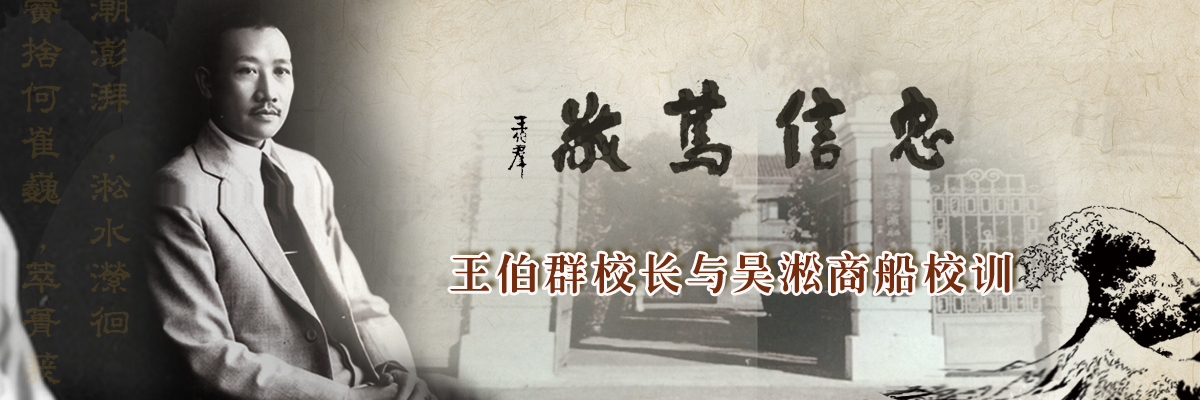
\includegraphics[width=10cm]{shmtu-school-motto}
	\caption{王伯群校长与吴淞商船校训}
	\label{fig:shmtu-school-motto}
\end{figure}

\begin{figure}[!htp]
	\centering
	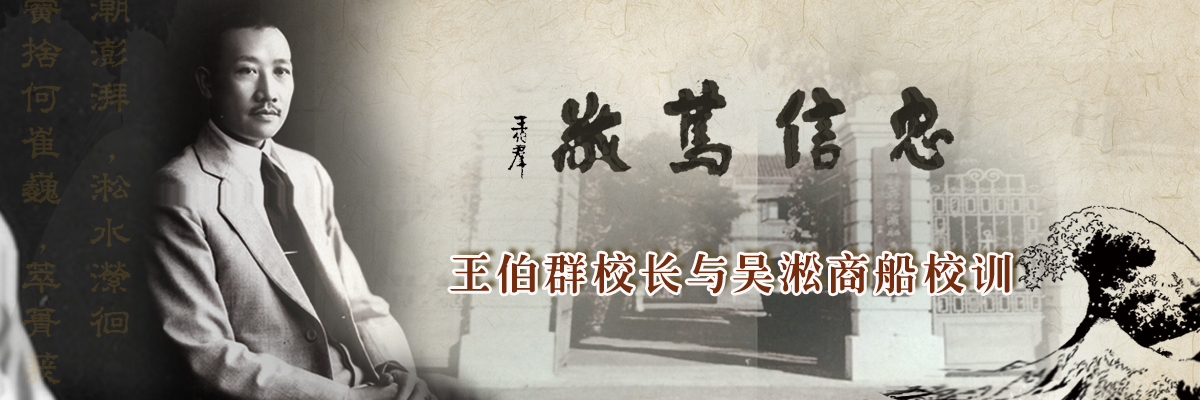
\includegraphics[width=10cm]{shmtu-school-motto}
	\bicaption{王伯群校长与吴淞商船校训}{President Wang Boqun and the school motto of WuSong Merchant Shipping}
	\label{fig:shmtu-school-motto-2}
\end{figure}

\subsection{多个图形}

简单插入多个图形的例子如图~\ref{fig:parallel-1} 所示。这两个水平并列放置的子图共用一个图形计数器,没有各自的子图题。

\begin{figure}[!htp]
  \centering
  
\includegraphics[height=2cm]{images/shmtu-badge}
  \hspace{1cm}
  
\includegraphics[height=2cm]{images/shmtu-badge}
  \caption{上海海事大学校徽}
  \label{fig:parallel-1}
\end{figure}

如果多个图形相互独立,并不共用一个图形计数器,那么用 \cs{minipage} 或者\cs{parbox} 就可以,如图~\ref{fig:parallel-2-1} 与图~\ref{fig:parallel-2-2}。

\begin{figure}[!htp]
  \begin{minipage}{0.48\textwidth}
  	\centering
    
\includegraphics[height=1.5cm]{images/shmtu-badge.jpg}
    \caption{并排第一个图}
    \label{fig:parallel-2-1}
  \end{minipage}
  \hfill
  \begin{minipage}{0.48\textwidth}
    \centering
    
\includegraphics[height=1.5cm]{images/shmtu-badge.jpg}
    \caption{并排第二个图}
    \label{fig:parallel-2-2}
  \end{minipage}
\end{figure}

如果要为共用一个计数器的多个子图添加子图注,那么使用\cs{subcaptionbox}(双语图注使用\cs{bisubcaptionbox})并排子图,子图注置于子图之下,子图号用 (a)、(b)、(c)等表示。如图~\ref{fig:subcaptionbox}、图~\ref{fig:subcaptionbox-a}、图~\ref{fig:subcaptionbox-b}、图~\ref{fig:subcaptionbox-c}所示。

\begin{figure}[!htp]
  \subcaptionbox{上海海事大学校徽\label{fig:subcaptionbox-a}}%
	[0.5\textwidth]{%
	  
\includegraphics[height=1.5cm]{images/shmtu-badge}
	}
  \hfill
  \subcaptionbox{上海海事大学校名\label{fig:subcaptionbox-b}}%
    [0.5\textwidth]{%
	  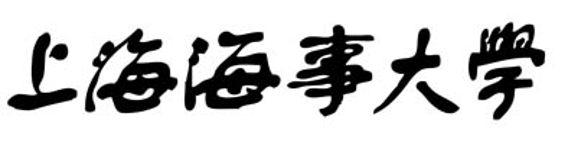
\includegraphics[width=0.5\textwidth]{images/shmtu-name}
	}
  \hfill
  \subcaptionbox{上海海事大学校徽\label{fig:subcaptionbox-c}}%
    [\textwidth]{%
	  
\includegraphics[height=1.5cm]{images/shmtu-badge}
  }
  \caption{共用一个计数器的多个子图图注}
  \label{fig:subcaptionbox}
\end{figure}

\section{表格}

\subsection{基本表格}

编排表格应简单明了,表达一致,明晰易懂,表文呼应、内容一致。表注置于表上,研究生学位论文可以用中、英文两种文字居中排写,中文在上,也可以只用中文。

表格的编排采用国际通行的三线表\footnote{三线表,以其形式简洁、功能分明、阅读方便而在科技论文中被推荐使用。三线表通常只有 3 条线,即顶线、底线和栏目线,没有竖线。}。三线表可以使用 \pkg{booktabs} 提供的 \cs{toprule}、\cs{midrule} 和 \cs{bottomrule}。它们与 \pkg{longtable} 能很好的配合使用。

\begin{table}[!htp]
  \centering
  \caption[一个标准的三线表]{一个标准的三线表\footnotemark}
  \label{tab:firstone}
  \begin{tabular}{llr}  
    \toprule
    \multicolumn{2}{c}{Item} \\
    \cmidrule(r){1-2}
    Animal    & Description & Price (\$) \\
    \midrule
    Gnat      & per gram    & 13.65      \\
              &    each     & 0.01       \\
    Gnu       & stuffed     & 92.50      \\
    Emu       & stuffed     & 33.33      \\
    Armadillo & frozen      & 8.99       \\
    \bottomrule
  \end{tabular}
\end{table}
\footnotetext{这个例子来自
  \href{https://mirrors.sjtug.sjtu.edu.cn/ctan/macros/latex/contrib/booktabs/booktabs.pdf}%
  {《Publication quality tables in LaTeX》}(\pkg{booktabs} 宏包的文档)。这也是
  一个在表格中使用脚注的例子,请留意与 \pkg{threeparttable} 实现的效果有何不
  同。}
  
\subsection{复杂表格}

我们经常会在表格下方标注数据来源,或者对表格里面的条目进行解释。可以用\pkg{threeparttable} 实现带有脚注的表格,如表~\ref{tab:footnote}。

\begin{table}[!htpb]
  \bicaption{一个带有脚注的表格的例子}{A Table with footnotes}
  \label{tab:footnote}
  \centering
  \begin{threeparttable}[b]
     \begin{tabular}{ccd{4}cccc}
      \toprule
      \multirow{2}*{total} & \multicolumn{2}{c}{20\tnote{a}} & \multicolumn{2}{c}{40} & \multicolumn{2}{c}{60} \\
      \cmidrule(lr){2-3}\cmidrule(lr){4-5}\cmidrule(lr){6-7}
      & www & \multicolumn{1}{c}{k} & www & k & www & k \\ % 使用说明符 d 的列会自动进入数学模式,使用 \multicolumn 对文字表头做特殊处理
      \midrule
      & $\underset{(2.12)}{4.22}$ & 120.0140\tnote{b} & 333.15 & 0.0411 & 444.99 & 0.1387 \\
      & 168.6123 & 10.86 & 255.37 & 0.0353 & 376.14 & 0.1058 \\
      & 6.761    & 0.007 & 235.37 & 0.0267 & 348.66 & 0.1010 \\
      \bottomrule
    \end{tabular}
    \begin{tablenotes}
      \item [a] the first note.% or \item [a]
      \item [b] the second note.% or \item [b]
    \end{tablenotes}
  \end{threeparttable}
\end{table}

\zhlipsum[1]

如某个表需要转页接排,可以用 \pkg{longtable} 实现。接排时表注省略,表头应重复书写,并在右上方写“续表 xx”,如表~\ref{tab:grid_mlmmh}。

\begin{longtable}[c]{c*{3}{r}}
  \caption[高变网格的可行三元组]{高变网格的可行三元组, MLMMH.}
  \label{tab:grid_mlmmh} \\
  % 表头
  \toprule
  \multicolumn{1}{c}{Time (s)} & \multicolumn{1}{c}{Triple chosen} & \multicolumn{1}{c}{Other feasible triples} \\
  \midrule
  \endfirsthead
	
  % 续表
  \multicolumn{3}{r}{续表~\thetable} \\
  \toprule
  % 续表表头
  \multicolumn{1}{c}{\textbf{Time (s)}} & \multicolumn{1}{c}{\textbf{Triple chosen}} & \multicolumn{1}{c}{\textbf{Other feasible triples}} \\ 
  \midrule
  \endhead

  \midrule
  \multicolumn{3}{r}{续下页} \\
  \endfoot
  
  \bottomrule
  \endlastfoot
  
0 & (1, 11, 13725) & (1, 12, 10980), (1, 13, 8235), (2, 2, 0), (3, 1, 0) \\
2745 & (1, 12, 10980) & (1, 13, 8235), (2, 2, 0), (2, 3, 0), (3, 1, 0) \\
5490 & (1, 12, 13725) & (2, 2, 2745), (2, 3, 0), (3, 1, 0) \\
8235 & (1, 12, 16470) & (1, 13, 13725), (2, 2, 2745), (2, 3, 0), (3, 1, 0) \\
10980 & (1, 12, 16470) & (1, 13, 13725), (2, 2, 2745), (2, 3, 0), (3, 1, 0) \\
13725 & (1, 12, 16470) & (1, 13, 13725), (2, 2, 2745), (2, 3, 0), (3, 1, 0) \\
16470 & (1, 13, 16470) & (2, 2, 2745), (2, 3, 0), (3, 1, 0) \\
19215 & (1, 12, 16470) & (1, 13, 13725), (2, 2, 2745), (2, 3, 0), (3, 1, 0) \\
21960 & (1, 12, 16470) & (1, 13, 13725), (2, 2, 2745), (2, 3, 0), (3, 1, 0) \\
24705 & (1, 12, 16470) & (1, 13, 13725), (2, 2, 2745), (2, 3, 0), (3, 1, 0) \\
27450 & (1, 12, 16470) & (1, 13, 13725), (2, 2, 2745), (2, 3, 0), (3, 1, 0) \\
30195 & (2, 2, 2745) & (2, 3, 0), (3, 1, 0) \\
32940 & (1, 13, 16470) & (2, 2, 2745), (2, 3, 0), (3, 1, 0) \\
35685 & (1, 13, 13725) & (2, 2, 2745), (2, 3, 0), (3, 1, 0) \\
38430 & (1, 13, 10980) & (2, 2, 2745), (2, 3, 0), (3, 1, 0) \\
41175 & (1, 12, 13725) & (1, 13, 10980), (2, 2, 2745), (2, 3, 0), (3, 1, 0) \\
43920 & (1, 13, 10980) & (2, 2, 2745), (2, 3, 0), (3, 1, 0) \\
46665 & (2, 2, 2745) & (2, 3, 0), (3, 1, 0) \\
49410 & (2, 2, 2745) & (2, 3, 0), (3, 1, 0) \\
52155 & (1, 12, 16470) & (1, 13, 13725), (2, 2, 2745), (2, 3, 0), (3, 1, 0) \\
54900 & (1, 13, 13725) & (2, 2, 2745), (2, 3, 0), (3, 1, 0) \\
57645 & (1, 13, 13725) & (2, 2, 2745), (2, 3, 0), (3, 1, 0) \\
60390 & (1, 12, 13725) & (2, 2, 2745), (2, 3, 0), (3, 1, 0) \\
63135 & (1, 13, 16470) & (2, 2, 2745), (2, 3, 0), (3, 1, 0) \\
65880 & (1, 13, 16470) & (2, 2, 2745), (2, 3, 0), (3, 1, 0) \\
68625 & (2, 2, 2745) & (2, 3, 0), (3, 1, 0) \\
71370 & (1, 13, 13725) & (2, 2, 2745), (2, 3, 0), (3, 1, 0) \\
74115 & (1, 12, 13725) & (2, 2, 2745), (2, 3, 0), (3, 1, 0) \\
76860 & (1, 13, 13725) & (2, 2, 2745), (2, 3, 0), (3, 1, 0) \\
79605 & (1, 13, 13725) & (2, 2, 2745), (2, 3, 0), (3, 1, 0) \\
82350 & (1, 12, 13725) & (2, 2, 2745), (2, 3, 0), (3, 1, 0) \\
85095 & (1, 12, 13725) & (1, 13, 10980), (2, 2, 2745), (2, 3, 0), (3, 1, 0) \\
87840 & (1, 13, 16470) & (2, 2, 2745), (2, 3, 0), (3, 1, 0) \\
\end{longtable}


\section{算法环境}

算法环境可以使用 \pkg{algorithms} 宏包或者较新的 \pkg{algorithm2e} 实现。算法~\ref{algo:algorithm} 是一个使用 \pkg{algorithm2e} 的例子。关于排版算法环境的具体方法,请阅读相关宏包的官方文档\footnote{\url{http://tug.ctan.org/macros/latex/contrib/algorithm2e/doc/algorithm2e.pdf}}。

\begin{algorithm}
  \DontPrintSemicolon % Some LaTeX compilers require you to use \dontprintsemicolon instead
  \KwIn{A finite set $A=\{a_1, a_2, \ldots, a_n\}$ of integers}
  \KwOut{The largest element in the set}
  
  $max \gets a_1$\;
  \For{$i \gets 2$ \textbf{to} $n$} {
    \eIf{$a_i > max$} {
      $max \gets a_i$\;
    }{
      pass\;
    }
  }
  \Return{$max$}\;
  \caption{{\sc Max} finds the maximum number}
  \label{algo:algorithm}
\end{algorithm}

\section{代码环境}

我们可以在论文中插入算法,但是不建议插入大段的代码。如果确实需要插入代码,建议使用 \pkg{listings} 宏包。

\begin{codeblock}[language=Python]
# -*- coding: utf-8 -*-
import click

from app.extensions import db
from app.models import Role


def register_commands(app):
    @app.cli.command()
    @click.option('--drop', is_flag=True, help='删除之前的表后再初始化.')
    def initdb(drop):
        """初始化数据库."""
        if drop:
            click.confirm('执行该命令将会删除当前数据库,确定要执行吗?', abort=True)
            db.drop_all()
            click.echo('删除所有表.')
        db.create_all()
        click.echo('初始化数据库.')

    @app.cli.command()
    def init():
        """初始化项目"""
        click.echo('初始化数据库...')
        db.create_all()
        
        click.echo('初始化用户角色与权限...')
        Role.init_role()

        click.echo('初始化完毕.')
\end{codeblock}


	\chapter{数学符号与引用文献的标注}

\section{数学}

\subsection{数字与单位}

宏包 \pkg{siunitx} \footnote{\url{http://tug.ctan.org/macros/latex/exptl/siunitx/siunitx.pdf}}提供了更好的数字和单位支持,具体请查看相关文档:
\begin{itemize}
	\item \num{12345,67890}
	\item \num{1+-2i}
	\item \num{.3e45}
	\item \num{1.654 x 2.34 x 3.430}
	\item \si{kg.m.s^{-1}}
	\item \si{\kilogram\metre\per\second}
	\item \si[per-mode=symbol]{\kilogram\metre\per\second}
	\item \si[per-mode=symbol]{\kilogram\metre\per\ampere\per\second}
	\item \numlist{10;20;30}
	\item \SIlist{0.13;0.67;0.80}{\milli\metre}
	\item \numrange{10}{20}
    \item \SIrange{10}{20}{\degreeCelsius}
	\item \SIrange{0.13}{0.67}{\milli\metre}
	\item \ang{10}
	\item \ang{12.3}
	\item \ang{4,5}
	\item \ang{1;2;3}
	\item \ang{;;1}
	\item \ang{+10;;}
	\item \ang{-0;1;}
\end{itemize}

\subsection{数学符号和公式}

本小节仅演示基本用法,数学符号、公式、数组的详细内容,请查看文档\footnote{\url{https://en.wikibooks.org/wiki/LaTeX/Mathematics}}。

微分符号 $\dif$ 应使用正体,本模板提供了 \cs{dif} 命令。除此之外,模板还提供了一些命令方便使用:
\begin{itemize}
  \item 圆周率 $\uppi$:\verb|\uppi|
  \item 自然对数的底 $\upe$:\verb|\upe|
  \item 虚数单位 $\upi$, $\upj$:\verb|\upi| \verb|\upj|
\end{itemize}

公式应另起一行居中排版。公式后应注明编号,按章顺序编排,编号右端对齐。

\begin{equation}
	\cos (2\theta) = \cos^2 \theta - \sin^2 \theta
\end{equation}

\begin{equation}
  \frac{\dif^2 u}{\dif t^2} = \int f(x) \dif x.
\end{equation}

公式末尾是需要添加标点符号的,至于用逗号还是句号,取决于公式下面一句是接着公式说的,还是另起一句。

\begin{equation}
	\frac{2h}{\pi}\int_{0}^{\infty}\frac{\sin\left( \omega\delta \right)}{\omega}
	\cos\left( \omega x \right) \dif\omega = 
	\begin{cases}
		h, \ \left| x \right| < \delta, \\
		\frac{h}{2}, \ x = \pm \delta, \\
		0, \ \left| x \right| > \delta.
	\end{cases}
\end{equation}

公式较长时最好在等号“$=$”处转行。
\begin{align}
    & I (X_3; X_4) - I (X_3; X_4 \mid X_1) - I (X_3; X_4 \mid X_2) \nonumber \\
  = & [I (X_3; X_4) - I (X_3; X_4 \mid X_1)] - I (X_3; X_4 \mid \tilde{X}_2) \\
  = & I (X_1; X_3; X_4) - I (X_3; X_4 \mid \tilde{X}_2).
\end{align}

如果在等号处转行难以实现,也可在 $+$、$-$、$\times$、$\div$运算符号处转行,转行时运算符号仅书写于转行式前,不重复书写。
\begin{multline}
  \frac{1}{2} \Delta (f_{ij} f^{ij}) =
    2 \left(\sum_{i<j} \chi_{ij}(\sigma_{i} - \sigma_{j})^{2}
    + f^{ij} \nabla_{j} \nabla_{i} (\Delta f) \right. \\
  \left. + \nabla_{k} f_{ij} \nabla^{k} f^{ij} +
    f^{ij} f^{k} \left[2\nabla_{i}R_{jk}
    - \nabla_{k} R_{ij} \right] \vphantom{\sum_{i<j}} \right).
\end{multline}


需要在文中引用某个指定公式,如公式~\ref{eq:array}所示:

\begin{equation}
	A_{m,n} = 
	\begin{pmatrix}
		a_{1,1} & a_{1,2} & \cdots & a_{1,n} \\
		a_{2,1} & a_{2,2} & \cdots & a_{2,n} \\
		\vdots  & \vdots  & \ddots & \vdots  \\
		a_{m,1} & a_{m,2} & \cdots & a_{m,n} 
	\end{pmatrix}\label{eq:array}
\end{equation}

\subsection{定理环境}

示例文件中使用 \pkg{ntheorem} 宏包配置了定理、引理和证明等环境。用户也可以使用\pkg{amsthm} 宏包。

这里举一个“定理”和“证明”的例子:
\begin{theorem}[留数定理]\label{thm:res}
  假设 $U$ 是复平面上的一个单连通开子集,$a_1, \ldots, a_n$ 是复平面上有限个点,
  $f$ 是定义在 $U \backslash \{a_1, \ldots, a_n\}$ 上的全纯函数,如果 $\gamma$
  是一条把 $a_1, \ldots, a_n$ 包围起来的可求长曲线,但不经过任何一个 $a_k$,并且
  其起点与终点重合,那么:

  \begin{equation}
    \label{eq:res}
    \ointop_\gamma f(z)\, \dif z = 2\uppi \upi \sum_{k=1}^n \operatorname{I}(\gamma, a_k) \operatorname{Res}(f, a_k).
  \end{equation}

  如果 $\gamma$ 是若尔当曲线,那么 $\operatorname{I}(\gamma, a_k) = 1$,因此:

  \begin{equation}
    \label{eq:resthm}
    \ointop_\gamma f(z)\, \dif z = 2\uppi \upi \sum_{k=1}^n \operatorname{Res}(f, a_k).
  \end{equation}

  在这里,$\operatorname{Res}(f, a_k)$ 表示 $f$ 在点 $a_k$ 的留数,
  $\operatorname{I}(\gamma, a_k)$ 表示 $\gamma$ 关于点 $a_k$ 的卷绕数。卷绕数是
  一个整数,它描述了曲线 $\gamma$ 绕过点 $a_k$ 的次数。如果 $\gamma$ 依逆时针方
  向绕着 $a_k$ 移动,卷绕数就是一个正数,如果 $\gamma$ 根本不绕过 $a_k$,卷绕数
  就是零。
\end{theorem}

定理~\ref{thm:res} 的证明。
	
\begin{proof}
  首先,由\dots

  其次,\dots

  所以,\dots
\end{proof}

\section{引用文献的标注}

按照上海海事大学的要求,参考文献外观应符合国标 GB/T 7714 的要求。具体建议使用87版标准,由于这个版本太老(1988年1月1日实施),故本模版使用该国标下最新的2015版标准。本模版使用 \BibLaTeX\ 配合 \pkg{biblatex-gb7714-2015} 样式包\footnote{\url{https://www.ctan.org/pkg/biblatex-gb7714-2015}}控制参考文献的输出样式,后端采用 \pkg{biber} 管理文献。

请注意 \pkg{biblatex-gb7714-2015} 宏包 2016 年 9 月才加入 CTAN,如果你使用的\TeX\ 系统版本较旧,可能没有包含 \pkg{biblatex-gb7714-2015} 宏包,需要手动安装。\BibLaTeX\ 与 \pkg{biblatex-gb7714-2015} 目前在活跃地更新,为避免一些兼容性问题,推荐使用较新的版本。

正文中引用参考文献时,使用 \verb|\cite{key1,key2,key3...}| 可以产生“上标引用的参考文献”。使用\verb|\parencite{key1, key2, key3...}| 则可以产生水平引用的参考文献。建议将bibtex文献中的标示都改为英文,以免出现不兼容现象。

具体请看下面的例子,将会穿插使用水平的和上标的参考文献:Chen调查了用于语言n-gram建模的平滑模型的最广泛使用的算法,并提出了改进的语言模型平滑度,从而改善了语音识别性能\cite{chen1999empirical};SRILM是C ++库,可执行程序和帮助程序脚本的集合,旨在允许为语音识别和其他应用程序生成统计语言模型并进行实验\cite{stolcke2002srilm}。Sundermeyer、Soutner、王毅、梁军等人将LSTM应用到自然语言处理领域,并获得了不错的实验结果\cite{sundermeyer2012lstm, soutner2013application, wangyi2018, liangjun2015}。文献\parencite{sundermeyer2012lstm, soutner2013application, wangyi2018, liangjun2015}中均使用LSTM神经网络架构。

当需要将参考文献条目加入到文献表中但又不在正文中引用,可以使用\verb|\nocite{key1,key2,key3...}|。或者使用 \verb|\nocite{*}| 将参考文献数据库中的所有条目加入到文献表中。\nocite{*}

	\chapter{结论}

在这里祝大家写论文时文如泉涌,下笔有神,答辩顺利。

\zhlipsum[12-16]
	
	% 致谢
	\begin{acknowledgements}
	感谢 \LaTeX 开源项目组;
	
	感谢 \href{https://github.com/CTeX-org/ctex-kit}{CTeX-kit}提供了 LaTeX 的中文支持;
	
	感谢上海交大大学的\href{https://github.com/sjtug}{sjtug}项目组提供的开源模版,为本模版提供了基础代码。
\end{acknowledgements}

	
	% 参考文献
	\printbibliography[heading=bibintoc]
	
	% 使用英文字母对附录编号
	\appendix
	\chapter{Maxwell Equations}

选择二维情况,有如下的偏振矢量:
\begin{subequations}
  \begin{align}
    {\bf E} &= E_z(r, \theta) \hat{\bf z}, \\
    {\bf H} &= H_r(r, \theta) \hat{\bf r} + H_\theta(r, \theta) \hat{\bm\theta}.
  \end{align}
\end{subequations}
对上式求旋度:
\begin{subequations}
  \begin{align}
    \nabla \times {\bf E} &= \frac{1}{r} \frac{\partial E_z}{\partial\theta}
      \hat{\bf r} - \frac{\partial E_z}{\partial r} \hat{\bm\theta}, \\
    \nabla \times {\bf H} &= \left[\frac{1}{r} \frac{\partial}{\partial r}
      (r H_\theta) - \frac{1}{r} \frac{\partial H_r}{\partial\theta} \right]
      \hat{\bf z}.
  \end{align}
\end{subequations}
因为在柱坐标系下,$\overline{\overline\mu}$ 是对角的,所以 Maxwell 方程组中电场
$\bf E$ 的旋度:
\begin{subequations}
  \begin{align}
    & \nabla \times {\bf E} = \upi \omega {\bf B}, \\
    & \frac{1}{r} \frac{\partial E_z}{\partial\theta} \hat{\bf r} -
      \frac{\partial E_z}{\partial r}\hat{\bm\theta} = \upi \omega \mu_r H_r
      \hat{\bf r} + \upi \omega \mu_\theta H_\theta \hat{\bm\theta}.
  \end{align}
\end{subequations}
所以 $\bf H$ 的各个分量可以写为:
\begin{subequations}
  \begin{align}
    H_r &= \frac{1}{\upi \omega \mu_r} \frac{1}{r}
      \frac{\partial E_z}{\partial\theta}, \\
    H_\theta &= -\frac{1}{\upi \omega \mu_\theta}
      \frac{\partial E_z}{\partial r}.
  \end{align}
\end{subequations}
同样地,在柱坐标系下,$\overline{\overline\epsilon}$ 是对角的,所以 Maxwell 方程
组中磁场 $\bf H$ 的旋度:
\begin{subequations}
  \begin{align}
    & \nabla \times {\bf H} = -\upi \omega {\bf D}, \\
    & \left[\frac{1}{r} \frac{\partial}{\partial r}(r H_\theta) - \frac{1}{r}
      \frac{\partial H_r}{\partial\theta} \right] \hat{\bf z} = -\upi \omega
      {\overline{\overline\epsilon}} {\bf E} = -\upi \omega \epsilon_z E_z
      \hat{\bf z}, \\
    & \frac{1}{r} \frac{\partial}{\partial r}(r H_\theta) - \frac{1}{r}
      \frac{\partial H_r}{\partial\theta} = -\upi \omega \epsilon_z E_z.
  \end{align}
\end{subequations}
由此我们可以得到关于 $E_z$ 的波函数方程:
\begin{equation}
  \frac{1}{\mu_\theta \epsilon_z} \frac{1}{r} \frac{\partial}{\partial r}
  \left(r \frac{\partial E_z}{\partial r} \right) + \frac{1}{\mu_r \epsilon_z}
  \frac{1}{r^2} \frac{\partial^2E_z}{\partial\theta^2} +\omega^2 E_z = 0.
\end{equation}

	\chapter{绘制流程图}

图~\ref{fig:flow_chart} 是一张流程图示意。使用 \pkg{tikz} 环境,搭配四种预定义节点(\verb+startstop+、\verb+process+、\verb+decision+和\verb+io+),可以容易地绘
制出流程图。

\begin{figure}[!htp]
  \centering
  \resizebox{6cm}{!}{\begin{tikzpicture}[node distance=2cm]
    \node (pic) [startstop] {待测图片};
    \node (bg) [io, below of=pic] {读取背景};
    \node (pair) [process, below of=bg] {匹配特征点对};
    \node (threshold) [decision, below of=pair, yshift=-0.5cm] {多于阈值};
    \node (clear) [decision, right of=threshold, xshift=3cm] {清晰?};
    \node (capture) [process, right of=pair, xshift=3cm, yshift=0.5cm] {重采};
    \node (matrix_p) [process, below of=threshold, yshift=-0.8cm] {透视变换矩阵};
    \node (matrix_a) [process, right of=matrix_p, xshift=3cm] {仿射变换矩阵};
    \node (reg) [process, below of=matrix_p] {图像修正};
    \node (return) [startstop, below of=reg] {配准结果};
     
    %连接具体形状
    \draw [arrow](pic) -- (bg);
    \draw [arrow](bg) -- (pair);
    \draw [arrow](pair) -- (threshold);

    \draw [arrow](threshold) -- node[anchor=south] {否} (clear);

    \draw [arrow](clear) -- node[anchor=west] {否} (capture);
    \draw [arrow](capture) |- (pic);
    \draw [arrow](clear) -- node[anchor=west] {是} (matrix_a);
    \draw [arrow](matrix_a) |- (reg);

    \draw [arrow](threshold) -- node[anchor=east] {是} (matrix_p);
    \draw [arrow](matrix_p) -- (reg);
    \draw [arrow](reg) -- (return);
\end{tikzpicture}}
  \caption{绘制流程图效果}
  \label{fig:flow_chart}
\end{figure}
	
	% 文后无编号部分
	\backmatter
	
	% 发表论文、获奖情况、申请专利、参与项目
	% 盲审论文中,发表学术论文及参与科研情况等仅以第几作者注明即可,不要出现作者或他人姓名
	\begin{publications}
  \item Chen H, Chan C~T. Acoustic cloaking in three dimensions using acoustic metamaterials[J]. Applied Physics Letters, 2007, 91:183518.
  \item Chen H, Wu B~I, Zhang B, et al. Electromagnetic Wave Interactions with a Metamaterial Cloak[J]. Physical Review Letters, 2007, 99(6):63903.
\end{publications}

% 盲审时显示
\begin{publications*}
  \item 第一作者. 中文核心期刊论文, 2007.
  \item 第一作者. EI 国际会议论文, 2006.
\end{publications*}
	\begin{awards}
	\item 上海海事大学硕士研究生入学奖学金四等奖
	\item 上海海事大学硕士研究生学业奖学金三等奖
\end{awards}

% 盲审时显示
\begin{awards*}
	\item 硕士研究生入学奖学金四等奖
	\item 硕士研究生学业奖学金三等奖
\end{awards*}
	\begin{patents}
	\item 第一发明人,“薛定谔的永动机”,专利申请号3141592653
\end{patents}

% 盲审时显示
\begin{patents*}
	\item 第一发明人,“薛定谔的永动机”,专利申请号xxxxxxxxxx
\end{patents*}

	\begin{projects}
	\item 参与301项目课题(2018年9月--2020年7月)
	\item 参与自然基金项目(2019年5月--2019年8月)
\end{projects}

\begin{projects*}
	\item 301项目“XXX”
	\item 自然基金项目“XXX”
\end{projects*}
	
\end{document}